\pr (2b) Vyberte funkciu, ktorej definičný obor je znázornený na obrázku.
\begin{multicols}{2}
\noindent
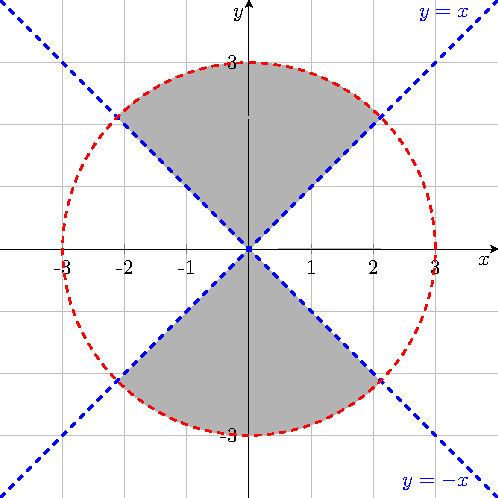
\includegraphics{kruznica3.pdf}

\noindent
\begin{itemize}
\item[a)] $\displaystyle f(x,y)= \ln{(9-x^2-y^2)}+\sqrt{x^2+y^2}$
\item[b)] $\displaystyle f(x,y)= \dfrac{\ln(9-x^2-y^2)}{\sqrt{x^2-y^2}}$
\item[c)] $\displaystyle f(x,y)= \sqrt{9-x^2-y^2}+\ln{(x^2-y^2)}$
\item[d)] $\displaystyle f(x,y)= \dfrac{\ln(9-x^2-y^2)}{\sqrt{y^2-x^2}}$
\end{itemize}
\end{multicols}
